\section{Desarrollo} 
\begin{itemize}

	\item a) Ejercicio 1 : Modelo Físico
		\begin{figure}[H]
		\begin{center}
		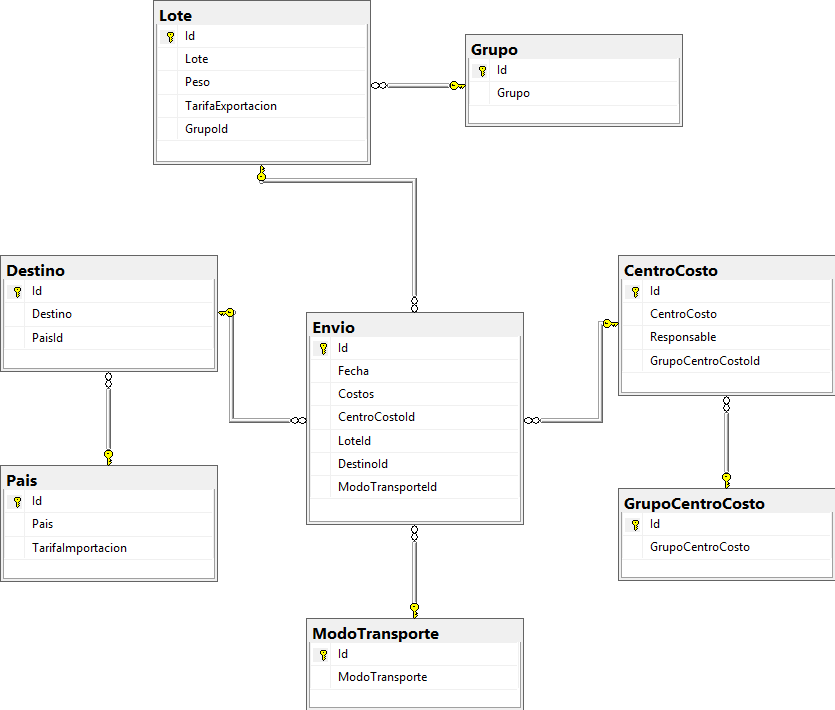
\includegraphics[width=18cm]{./Imagenes/imagen1}
		\end{center}
		\end{figure}

     	\item b) Ejercicio1: Modelo Dimensional
		\begin{figure}[H]
		\begin{center}
		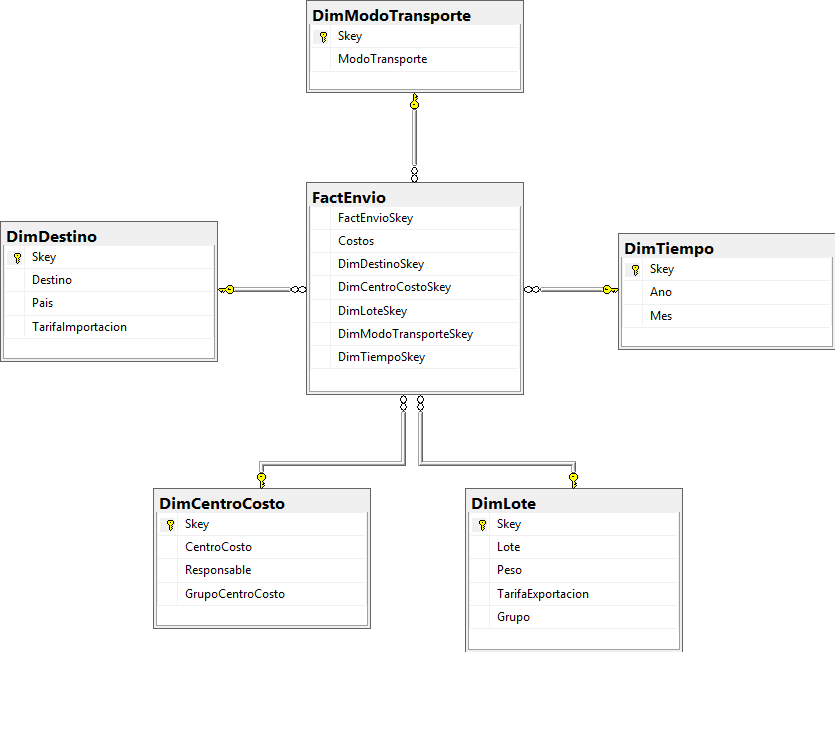
\includegraphics[width=18cm]{./Imagenes/imagen2}
		\end{center}
		\end{figure}
     

	\item c) Ejercicio 2 : Modelo Físico 
		\begin{figure}[H]
		\begin{center}
		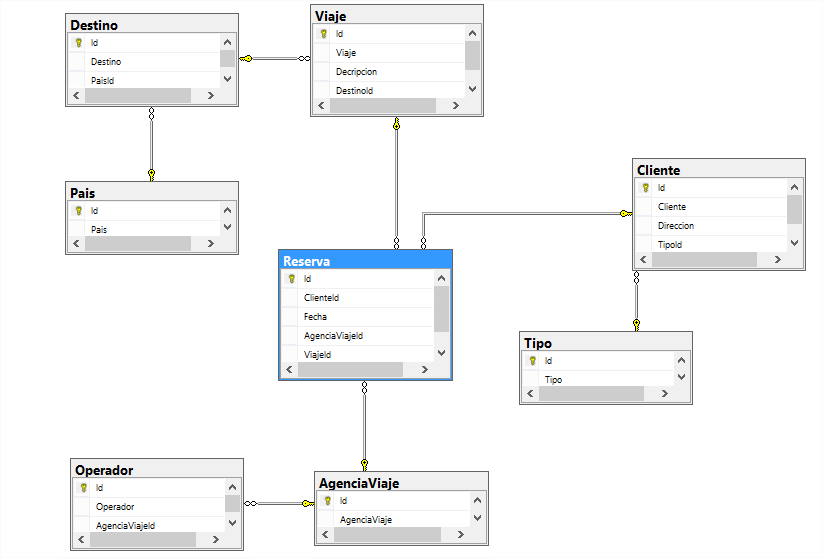
\includegraphics[width=18cm]{./Imagenes/imagen3}
		\end{center}
		\end{figure}
     
	\item d) Ejercicio 2:   Modelo Dimensional
		\begin{figure}[H]
		\begin{center}
		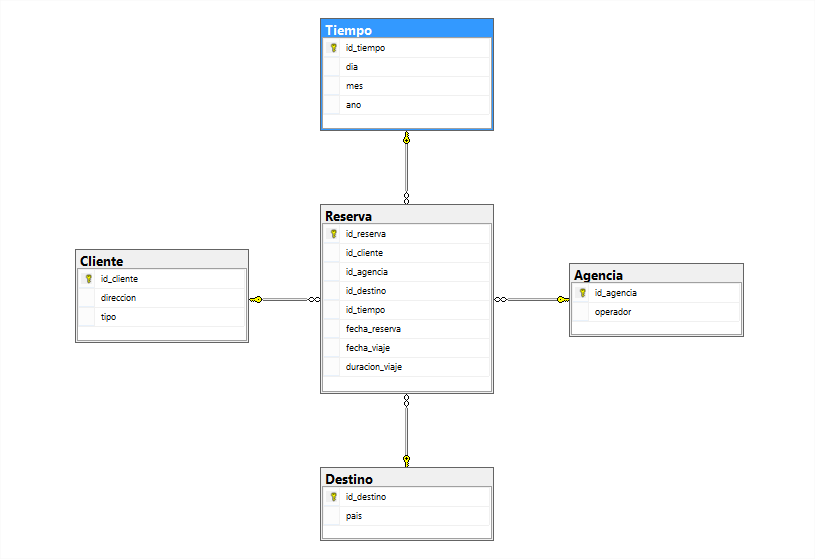
\includegraphics[width=18cm]{./Imagenes/imagen4}
		\end{center}
		\end{figure}
     
	\item e) Ejercicio 3:  Modelo Físico
		\begin{figure}[H]
		\begin{center}
		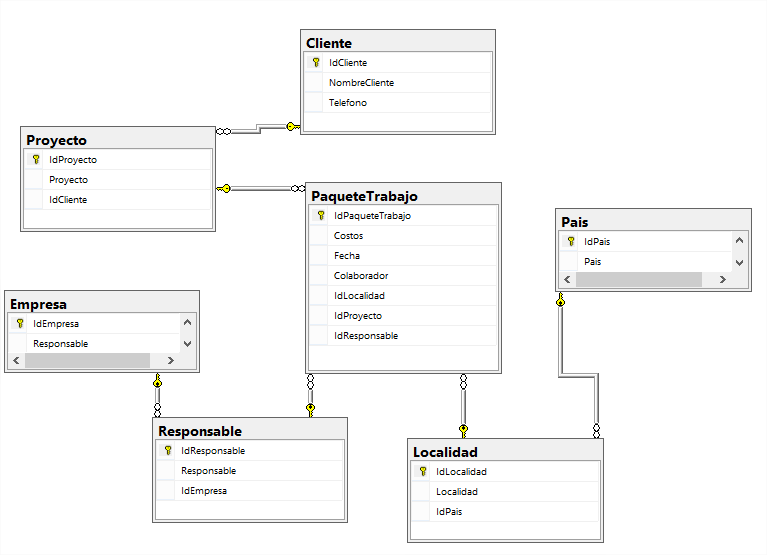
\includegraphics[width=18cm]{./Imagenes/imagen5}
		\end{center}
		\end{figure}
     
     
	\item f) Ejercicio 3:   Modelo Dimensional
		\begin{figure}[H]
		\begin{center}
		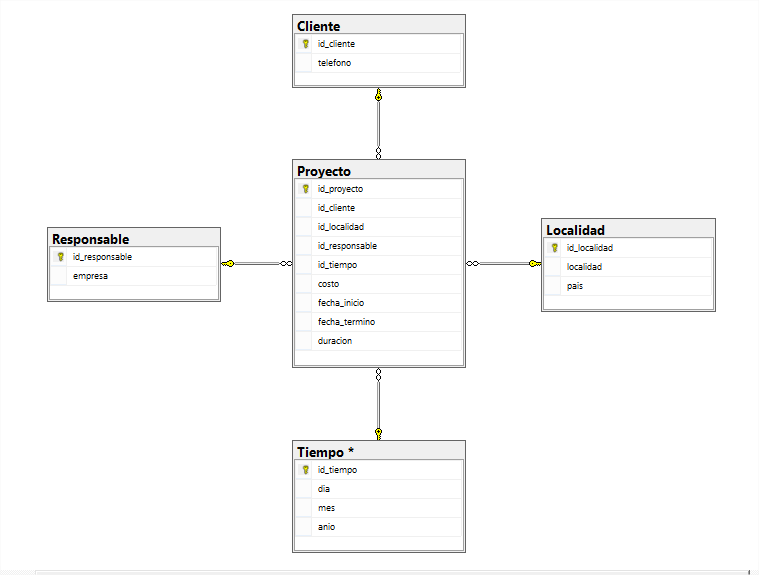
\includegraphics[width=18cm]{./Imagenes/imagen6}
		\end{center}
		\end{figure}
     



\end{itemize}
		